% -*- root: Proposal.tex -*-
\documentclass[Proposal.tex]{subfiles} 
\begin{document}
\chapter{Space-time DPG}
\label{sec:spacetime}
We summarize some completed work on space-time DPG. At the time of writing, Camellia does not officially support space-time computations, but we can fake it for 1D spatial problems by pretending the $y$-direction is time.
Complications arise when the PDE under consideration is parabolic (i.e. contains second derivatives in space, but only first derivatives in time). 
Mathematically, this leaves traces undefined on element edges without a spatial normal component. 
Practically, this means that I had to hack the Camellia code in order to support these ``spatial traces''.
We say that the code was ``hacked'' to indicate that we modified the code in an ``ugly'' manner in order to obtain the following results, 
but plan is to do this according to better software practices in the proposed work, since the current implementation is not very maintainable.

All of the following problems (unless otherwise noted) are run with the graph norm which is
simply defined from the adjoint of the system supplemented with $L^2$ terms to upgrade it to a full norm.

% \section{Pure Convection}
% The pure convection equation is 
% \begin{equation}
% \frac{\partial u}{\partial t}+\Div(\bfbeta u)=f\,,
% \end{equation}
% where $u$ is the unknown being convected, $\bfbeta$ is the convection vector, and $f$ is the source term.
% The convenient thing about pure convection is that the equation is the time dimension is basically indistinguishable from the spatial dimensions. 
% In fact, we can rewrite this in terms of a space-time divergence operator $\Divxt(u):=\Div(u)+\frac{\partial u}{\partial t}$:
% \[
% \Divxt\LRp{\vecttwo{\bfbeta}{1}u}=f\,.
% \]
% This means that spatially 1D space-time convection with convection vector $\alpha$ is identical to 2D steady convection with convection vector $\LRp{\alpha,1}^T$.
% We derive an ultra-weak DPG formulation for pure convection with $\bfbeta=\LRp{\alpha,1}^T$. 
% Multiplying by test function $v$ and integrating by parts over each element $K$, we get
% \begin{equation}
% -\LRp{\vecttwo{\alpha}{1}u,\Gradxt v}+\LRa{\hat t, v}=\LRp{f,v}\,,
% \end{equation}
% where $\hat t=\trace\LRp{\vecttwo{\alpha}{1}u}\cdot\bfn$.
% We omit numerical results in this case since pure convection was studied thoroughly in \cite{?}.

%   /$$   /$$                       /$$    
%  | $$  | $$                      | $$    
%  | $$  | $$  /$$$$$$   /$$$$$$  /$$$$$$  
%  | $$$$$$$$ /$$__  $$ |____  $$|_  $$_/  
%  | $$__  $$| $$$$$$$$  /$$$$$$$  | $$    
%  | $$  | $$| $$_____/ /$$__  $$  | $$ /$$
%  | $$  | $$|  $$$$$$$|  $$$$$$$  |  $$$$/
%  |__/  |__/ \_______/ \_______/   \___/  
%                                          
%                                          
%  
\section{Heat equation}
The simplest space-time problem we can consider where the the spatial and temporal dimensions are treated differently is the heat equation.
We start with a general $n$-dimensional spatial derivation and later simplify to spatially 1D with a few numerical experiments.

\subsection{Derivation}
Let $\Omega(t)\subset\mathbb{R}^d$ be the spatial domain with boundary $\partial\Omega$.
The heat equation is
\begin{equation}
	\frac{\partial u}{\partial t}-\mu\Delta u=f\,,\quad\bfx\in\Omega\,,\;t\in(t_0,T)
\end{equation}
where $u$ is unknown heat, $\epsilon$ is the diffusion scale, $f$ is the source term, $t_0$ is the start time, and $T$ is the final time.
Let $Q\subset\mathbb{R}^{d+1}$ denote the full space-time domain which is then tessellated into space-time elements $K$.

The second order formulation of the heat equation is really just a composition of Fourier's law and conservation of energy:
\begin{equation}
\label{eq:heatFirstOrder}
\begin{aligned}
\bfsigma-\epsilon\Grad u&=0\\
\frac{\partial u}{\partial t}-\Div\bfsigma&=f\,,
\end{aligned}
\end{equation}
where $\bfsigma$ is the heat flux.
The key insight that we will use over and over in the following problems is that we can rewrite our conservation equation
in terms of a space-time divergence operator: $\Divxt():=\Div()+\pt{()}$.
Our new system is then
\begin{equation}
\label{eq:heatFirstOrderSpaceTime}
\begin{aligned}
\frac{1}{\epsilon}\bfsigma-\Grad u&=0\\
\Divxt\vecttwo{-\bfsigma}{u}&=f\,.
\end{aligned}
\end{equation}
We now proceed with the standard DPG practice and multiply by test functions $\bftau$ and $v$ 
and integrate by parts over each space-time element $K$:
\begin{equation}
\label{eq:heatBF}
\begin{aligned}
\LRp{\frac{1}{\epsilon}\bfsigma,\bftau}+\LRp{u,\Div\bftau}-\LRa{\hat u,\bftau\cdot\bfn_x}&=0\\
-\LRp{\vecttwo{-\bfsigma}{u},\Gradxt v}+\LRa{\hat t,v}&=f\,,
\end{aligned}
\end{equation}
where
\begin{align*}
\hat u&:=\trace(u)\\
\hat t&:=\trace(-\bfsigma)\cdot\bfn_x+\trace(u)\cdot n_t
\end{align*}
are new unknowns that live on the mesh skeleton introduced by the integration by parts.
Note that the constitutive law was only integrated by parts over spatial dimensions, which means 
that ``spatial trace'' $\hat u$ only exists on mesh boundaries with a nonzero spatial normal component.
On the other hand, flux $\hat t$ exists on all mesh boundaries, but changes nature between pure spatial and temporal edges while taking on 
a mixed nature on slanted boundaries. We illustrate the support of these skeleton variables in Figure~\ref{fig:heatMesh}.

\begin{figure}[h!]
\begin{tikzpicture}[line cap=round,line join=round,>=triangle 45,x=2.0cm,y=2.0cm]
\clip(-0.7,-1.01) rectangle (5.27,2.29);
\draw (0,2)-- (0,0);
\draw (0,0)-- (1,0);
\draw (1,0)-- (4,0);
\draw (4,0)-- (5,0);
\draw (5,0)-- (5,2);
\draw (5,2)-- (3,2);
\draw (3,2)-- (2,2);
\draw (2,2)-- (0,2);
\draw (1,0)-- (1.5,1);
\draw (1.5,1)-- (2,2);
\draw (1.5,1)-- (3.5,1);
\draw (3,2)-- (3.5,1);
\draw (3.5,1)-- (4,0);
\draw (-0.21,0.9) node[anchor=south west] {$\hat u$};
\draw (4.82,0.9) node[anchor=south west] {$\hat u$};
\draw (3.5,0.45) node[anchor=south west] {$\hat u$};
\draw (1.0,0.45) node[anchor=south west] {$\hat u$};
\draw (1.5,1.4) node[anchor=south west] {$\hat u$};
\draw (3.0,1.4) node[anchor=south west] {$\hat u$};
\draw (0.05,0.9) node[anchor=south west] {$\hat t$};
\draw (1.40,0.45) node[anchor=south west] {$\hat t$};
\draw (3.79,0.45) node[anchor=south west] {$\hat t$};
\draw (2.47,1.0) node[anchor=south west] {$\hat t$};
\draw (3.33,1.4) node[anchor=south west] {$\hat t$};
\draw (1.89,1.4) node[anchor=south west] {$\hat t$};
\draw (5.07,0.9) node[anchor=south west] {$\hat t$};
\draw (4.44,0.0) node[anchor=south west] {$\hat t$};
\draw (2.46,0.0) node[anchor=south west] {$\hat t$};
\draw (0.45,0.0) node[anchor=south west] {$\hat t$};
\draw (2.44,1.7) node[anchor=south west] {$\hat t$};
\draw (0.76,1.7) node[anchor=south west] {$\hat t$};
\draw (4.21,1.7) node[anchor=south west] {$\hat t$};
\draw [->] (-0.5,-0.5) -- (-0.5,0);
\draw [->] (-0.5,-0.5) -- (0,-0.5);
\draw (-0.54,0.29) node[anchor=north west] {$t$};
\draw (0.07,-0.35) node[anchor=north west] {$x$};
\end{tikzpicture}
\caption{Support of flux and spatial trace variables}
\label{fig:heatMesh}
\end{figure}

% Let us say that $f\in\LQ$, then we seek $u$, and $\bfsigma$ such that $u,\,\bfsigma,\,\Grad u,\,\frac{\partial u}{\partial t}-\Div\bfsigma\in\LQ$.
% Notice that this is a weaker condition than saying $\frac{\partial u}{\partial t}\in\LQ$ and $\Div\bfsigma\in\LQ$.
% It helps to view $\bfU:=(-\bfsigma, u)$ as a group variable in space-time. 
% Then the last condition is telling us that $\Divxt\bfU\in\LQ$, or that $\bfU\in\HdivQ$.
% That is to say the normal component $-\bfsigma\cdot\bfn_x+u\cdot n_t$ (which we call the flux) is continuous across element faces, 
% where $\bfn=(\bfn_x,n_t)^T$ is the full space-time normal vector for element $K$.
% Now consider the condition that $\Grad u\in\LQ$.
% This implies that $u$ lives in a tensor product space of $H^1$ spatially and $L^2$ temporally and that
% $u\cdot n_t$ is continuous on element faces where $n_t$ is nonzero; we call this the spatial trace.

% Now that we understand which Sobolev spaces $u$ and $\bfsigma$ live in, we can proceed with a derivation of the space-time DPG formulation for this problem.
% We multiply the first equation in \eqref{eq:heatFirstOrder} by test function $\bftau$ and the second by $v$. Then we integrate by parts over each element:
% \begin{equation}
% \label{eq:heatBF}
% 	\begin{aligned}
% 		\LRp{\bfsigma,\bftau}+\epsilon\LRp{u,\Div\bftau}-\LRa{\hat u,\tau_n}&=0\\
% 		-\LRp{u,\frac{\partial v}{\partial t}}+\LRp{\bfsigma,\Grad v}-\LRa{\hat t,v}&=\LRp{f,v}\,,
% 	\end{aligned}
% \end{equation}
% where $\hat u$ is the spatial trace and $\hat t$ is the flux.
% The second equation could alternatively be written in terms of the group variable $\bfU$:
% \begin{equation}
% \label{heatBFAlt}
% -\LRp{\bfU,\Gradxt v}-\LRa{\hat t,v}=\LRp{f,v}\,.
% \end{equation}
% This alternate version emphasizes the definition of the flux: $\hat t=\trace\LRp{-\bfsigma}\cdot\bfn_x+\trace{(u)}\cdot n_t$.
% From \eqref{eq:heatBF} and \eqref{heatBFAlt} it is clear that $\bftau\in\HdivK$ where the divergence is taken only over spatial directions, and $v\in\HOneK$.
% Figure \ref{fig:heatMesh} illustrates the support for the fluxes and spatial traces. Notice that the fluxes live on all element boundaries, while the spatial traces only live on ``non-horizontal'' edges.

\subsection{Problems considered}
If we consider a domain $\Omega=[0,1]^2$ with an initial condition of $u=\cos(2\pi x)$ with zero flux conditions at the boundaries,
the exact solution is
\begin{equation*}
	u=\cos(2\pi x)e^{-4*\pi^2\epsilon t}\,.
\end{equation*}
We ran this with $\epsilon=10^{-2}$ on a sequence of uniform meshes and $p=2$ for the field representation of $u$. 
We were able to achieve the expected third order convergence as demonstrated in Figure \ref{fig:spaceTimeHeatConvergence}.

\begin{figure}[!ht]
	\centering
	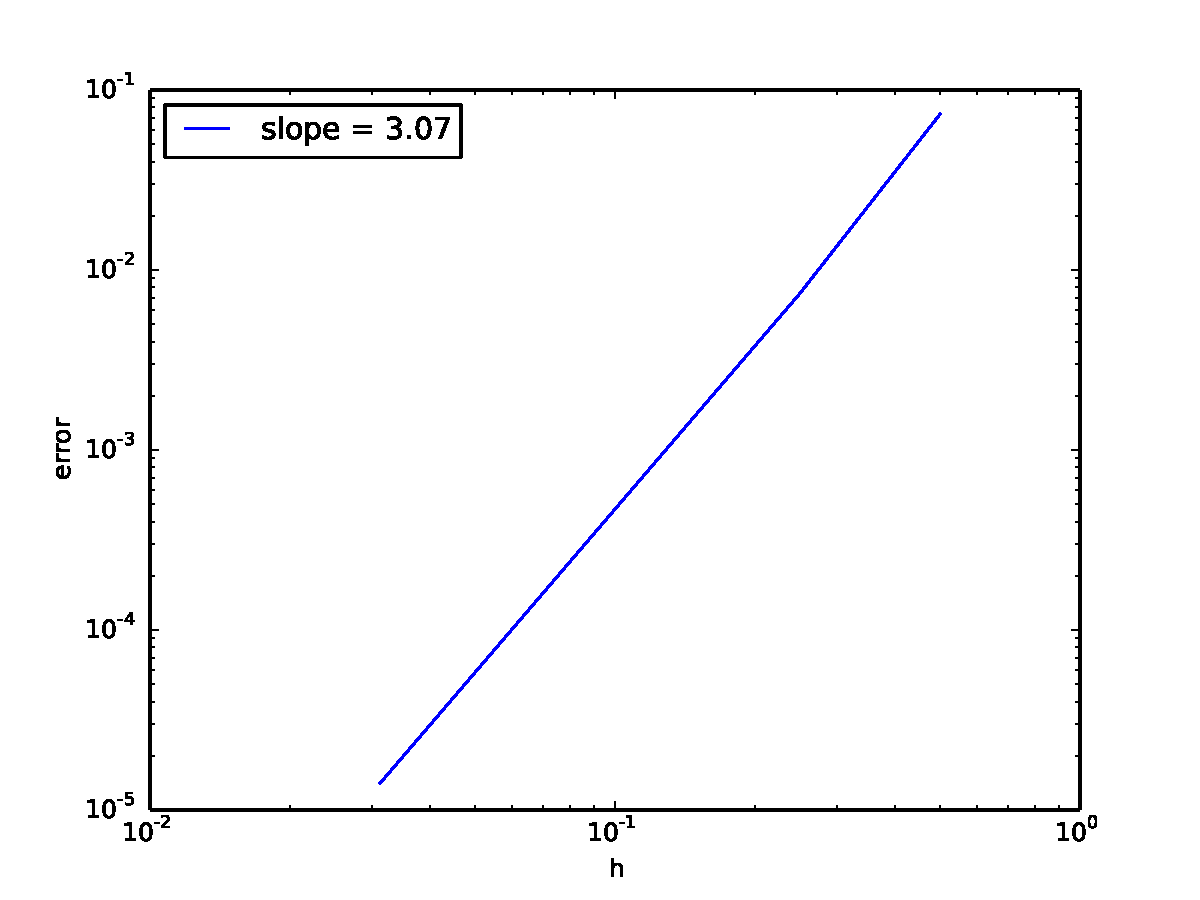
\includegraphics[width=0.7\textwidth]{SpaceTimeHeat/convergence}
	\caption{$L^2$ convergence of $u$ for the space-time heat equation}
	\label{fig:spaceTimeHeatConvergence}
\end{figure}

In order to demonstrate local space-time adaptivity we consider one more problem for the heat equation. 
On the same domain, and with the same boundary conditions as the previous example, we let the initial heat distribution be zero.
Then between $t=0.25$ and $t=0.5$ we turn on a pulse source term of one on $0.375\leq x\leq 0.625$. 
Starting from an initial mesh of $4x4$, we adaptively refine four times and obtain the results in Figure \ref{fig:spaceTimeHeatPulse}.
Notice that $\hat u$ in Figure \ref{fig:spaceTimeHeatuhat} only lives on vertical edges as was discussed earlier.
Also notice that the full mesh shown in Figure \ref{fig:spaceTimeHeatfhat} automatically adapts spatially and temporally to where features are rapidly changing. 

\begin{figure}[p]
\centering
\begin{subfigure}[t]{0.45\textwidth}
\centering
\includegraphics[width=\textwidth]{SpaceTimeHeat/PulseSource/u.png}
\caption{$u$}
\label{fig:spaceTimeHeatu}
\end{subfigure}
\begin{subfigure}[t]{0.45\textwidth}
\centering
\includegraphics[width=\textwidth]{SpaceTimeHeat/PulseSource/sigma.png}
\caption{$\sigma$}
\label{fig:spaceTimeHeatsigma}
\end{subfigure}
\begin{subfigure}[t]{0.45\textwidth}
\centering
\includegraphics[width=\textwidth]{SpaceTimeHeat/PulseSource/uhat.png}
\caption{$\hat u$}
\label{fig:spaceTimeHeatuhat}
\end{subfigure}
\begin{subfigure}[t]{0.45\textwidth}
\centering
\includegraphics[width=\textwidth]{SpaceTimeHeat/PulseSource/fhat.png}
\caption{$\hat t$}
\label{fig:spaceTimeHeatfhat}
\end{subfigure}
\caption{Pulsed space-time heat problem after 4 refinements}
\label{fig:spaceTimeHeatPulse}
\end{figure}

%    /$$$$$$                       /$$$$$$                      /$$                    
%   /$$__  $$                     /$$__  $$                    |__/                    
%  | $$  \__/  /$$$$$$  /$$$$$$$ | $$  \__/ /$$   /$$  /$$$$$$$ /$$  /$$$$$$  /$$$$$$$ 
%  | $$       /$$__  $$| $$__  $$| $$$$    | $$  | $$ /$$_____/| $$ /$$__  $$| $$__  $$
%  | $$      | $$  \ $$| $$  \ $$| $$_/    | $$  | $$|  $$$$$$ | $$| $$  \ $$| $$  \ $$
%  | $$    $$| $$  | $$| $$  | $$| $$      | $$  | $$ \____  $$| $$| $$  | $$| $$  | $$
%  |  $$$$$$/|  $$$$$$/| $$  | $$| $$      |  $$$$$$/ /$$$$$$$/| $$|  $$$$$$/| $$  | $$
%   \______/  \______/ |__/  |__/|__/       \______/ |_______/ |__/ \______/ |__/  |__/
%                                                                                      
%                                                                                      
%        
\section{Convection-Diffusion}
Transient convection-diffusion is identical to the heat equation with the addition of a convective term:
\begin{equation*}
\frac{\partial u}{\partial t}+\Div(\bfbeta u)-\epsilon\Delta u=f\,.
\end{equation*}
The $d$-dimensional transient convection-diffusion equations could be viewed as a $d+1$ steady convection-diffusion problem with zero diffusion in the time direction.

\subsection{Derivation}
As a first order system in space-time, this is
\begin{equation}
\label{eq:confusionFirstOrder}
\begin{aligned}
\frac{1}{\epsilon}\bfsigma-\Grad u&=0\\
\Divxt\vecttwo{\bfbeta u-\bfsigma}{u}&=f\,.
\end{aligned}
\end{equation}
% We can view the second equation as a full space-time divergence on group variable $\bfU:=\LRc{\bfbeta u-\bfsigma,u}$ as before:
% \begin{equation}
% 	\Divxt\LRp{\bfU}=f\,.
% \end{equation}
Multiplying \eqref{eq:confusionFirstOrder} by test functions, and integrating by parts over each element, we obtain the following bilinear form:
\begin{equation}
\label{eq:confusionBF}
	\begin{aligned}
		\LRp{\frac{1}{\epsilon}\bfsigma,\bftau}+\LRp{u,\Div\bftau}-\LRa{\hat u,\tau_n}&=0\\
		-\LRp{\vecttwo{\bfbeta u-\bfsigma}{u},\Gradxt v}+\LRa{\hat t,v}&=f\,,
		% -\LRp{u,\frac{\partial v}{\partial t}}-\LRp{\bfbeta u,\Grad v}+\LRp{\bfsigma,\Grad v}-\LRa{\hat t,v}&=\LRp{f,v}\,,
	\end{aligned}
\end{equation}
where now $\hat t=\trace\LRp{\bfbeta u-\bfsigma}\cdot\bfn_x+\trace(u)\cdot n_t$, and $\hat u$ is as before. Our test functions, $\bftau$ and $v$ live in the same spaces as for the heat equation.

\subsection{Problems considered}
Since space-time convection-diffusion is identical the heat equation with the addition of a convective term, we only pursue one numerical experiment to demonstrate that everything works as expected. 
This problem is inspired by the previous heat problem with the spatial domain extended to prevent the convected heat from impinging on the right wall.
It might be interesting to impose a zero boundary condition on $\hat u$ and watch a boundary layer build up on the right wall, 
but instead we enforce a zero flux condition and content ourselves with the inner layer that forms around the source pulse.
This is an arbitrary requirement necessitated by the ``hackish'' nature of this code.
We haven't taken the time to allow enforcement of Dirichlet boundary conditions on spatial fluxes, and since the code in this state was intended to be short-lived, it doesn't make sense to invest too heavily in adding features. 
Thus we enforce zero flux conditions on both walls as before. 
For this problem, the domain extends from $[0,1.5]\times[0,1]$ with the pulse occurring at $[0.25,0.5]\times[0.25,0.5]$.

\begin{figure}[p]
\centering
\begin{subfigure}[t]{0.45\textwidth}
\centering
\includegraphics[width=\textwidth]{SpaceTimeConfusion/u.png}
\caption{$u$}
\label{fig:spaceTimeConfusionu}
\end{subfigure}
\begin{subfigure}[t]{0.45\textwidth}
\centering
\includegraphics[width=\textwidth]{SpaceTimeConfusion/sigma.png}
\caption{$\sigma$}
\label{fig:spaceTimeConfusionsigma}
\end{subfigure}
\begin{subfigure}[t]{0.45\textwidth}
\centering
\includegraphics[width=\textwidth]{SpaceTimeConfusion/uhat.png}
\caption{$\hat u$}
\label{fig:spaceTimeConfusionuhat}
\end{subfigure}
\begin{subfigure}[t]{0.45\textwidth}
\centering
\includegraphics[width=\textwidth]{SpaceTimeConfusion/fhat.png}
\caption{$\hat t$}
\label{fig:spaceTimeConfusionfhat}
\end{subfigure}
\caption{Space-time convection-diffusion problem after 4 refinements}
\label{fig:spaceTimeConfusion}
\end{figure}

%   /$$$$$$$                                                             
%  | $$__  $$                                                            
%  | $$  \ $$ /$$   /$$  /$$$$$$   /$$$$$$   /$$$$$$   /$$$$$$   /$$$$$$$
%  | $$$$$$$ | $$  | $$ /$$__  $$ /$$__  $$ /$$__  $$ /$$__  $$ /$$_____/
%  | $$__  $$| $$  | $$| $$  \__/| $$  \ $$| $$$$$$$$| $$  \__/|  $$$$$$ 
%  | $$  \ $$| $$  | $$| $$      | $$  | $$| $$_____/| $$       \____  $$
%  | $$$$$$$/|  $$$$$$/| $$      |  $$$$$$$|  $$$$$$$| $$       /$$$$$$$/
%  |_______/  \______/ |__/       \____  $$ \_______/|__/      |_______/ 
%                                 /$$  \ $$                              
%                                |  $$$$$$/                              
%                                 \______/   
% \section{Viscous Burgers' Equation}
% We consider the viscous Burgers' equation as a simple nonlinear parabolic problem:
% \begin{equation*}
% 	\pt{u}+u\pd{u}{x}-\epsilon\ppd{u}{x}=0\,,
% \end{equation*}
% where $u$ is the quantity of interest and $\epsilon$ is the diffusion length scale.
% Again, this can be put as a first order system in space-time:
% \begin{equation*}
% \begin{aligned}
% 	\frac{1}{\epsilon}\bfsigma-\Grad u&=0\\
% 	\Divxt\vecttwo{u^2/2-\bfsigma}{u}&=0\,.
% \end{aligned}
% \end{equation*}

% \subsection{Derivation}
% The process is starting to get repetitive, but we again multiply by test functions and integrate by parts to get the following nonlinear system:
% \begin{equation*}
% \begin{aligned}
% 	\LRp{\frac{1}{\epsilon}\bfsigma,\bftau}+\LRp{u,\Div\bftau}-\LRa{\hat u,\tau_n}&=0\\
% 	-\LRp{\vecttwo{u^2/2-\bfsigma}{u},\Gradxt v}+\LRa{\hat t, v}&=0\,.
% \end{aligned}
% \end{equation*}

% \subsection{Problems considered}

%    /$$$$$$                                                                            /$$ /$$       /$$          
%   /$$__  $$                                                                          |__/| $$      | $$          
%  | $$  \__/  /$$$$$$  /$$$$$$/$$$$   /$$$$$$   /$$$$$$   /$$$$$$   /$$$$$$$  /$$$$$$$ /$$| $$$$$$$ | $$  /$$$$$$ 
%  | $$       /$$__  $$| $$_  $$_  $$ /$$__  $$ /$$__  $$ /$$__  $$ /$$_____/ /$$_____/| $$| $$__  $$| $$ /$$__  $$
%  | $$      | $$  \ $$| $$ \ $$ \ $$| $$  \ $$| $$  \__/| $$$$$$$$|  $$$$$$ |  $$$$$$ | $$| $$  \ $$| $$| $$$$$$$$
%  | $$    $$| $$  | $$| $$ | $$ | $$| $$  | $$| $$      | $$_____/ \____  $$ \____  $$| $$| $$  | $$| $$| $$_____/
%  |  $$$$$$/|  $$$$$$/| $$ | $$ | $$| $$$$$$$/| $$      |  $$$$$$$ /$$$$$$$/ /$$$$$$$/| $$| $$$$$$$/| $$|  $$$$$$$
%   \______/  \______/ |__/ |__/ |__/| $$____/ |__/       \_______/|_______/ |_______/ |__/|_______/ |__/ \_______/
%                                    | $$                                                                          
%                                    | $$                                                                          
%                                    |__/    
\section{Transient Compressible Navier-Stokes}
We make a large jump from convection-diffusion to the compressible Navier-Stokes equations.
The following discussion holds in any dimension, but the provided results are only for spatially 1D flows.
The compressible Navier-Stokes equations are
\begin{align}
\frac{\partial}{\partial t}\svectthree{\rho}{\rho\bfu}{\rho e_0}
+\Div\svectthree{\rho\bfu}{\rho\bfu\otimes\bfu+p\bfI-\mathbb{D}}{\rho\bfu e_0+\bfu p+\bfq-\bfu\cdot\mathbb{D}}
%TODO: Possible error above. cfd-online seems to have T^T
=\svectthree{f_c}{\bff_m}{f_e}\,,
\end{align}
where $\rho$ is the density, $\bfu$ is the velocity, $p$ is the pressure, $\bfI$ is the identity matrix,
$\mathbb{D}$ is the deviatoric stress tensor or viscous stress, $e_0$ is the total energy, $\bfq$ is the heat flux, 
and $f_c$, $\bff_m$, and $f_e$ are the source terms for the continuity, momentum, and energy equations, respectively.
Assuming Stokes hypothesis that $\lambda=-\frac{2}{3}\mu$, 
\begin{equation*}
	\mathbb{D}=2\mu\bfS^*=2\mu\LRs{\frac{1}{2}\LRp{\Grad\bfu+\LRp{\Grad\bfu}^T}-\frac{1}{3}\Div\bfu\bfI}\,,
\end{equation*}
where $\bfS^*$ is the trace-less viscous strain rate tensor.
The heat flux is given by Fourier's law:
\begin{equation*}
	\bfq=-C_p\frac{\mu}{Pr}\Grad T\,,
\end{equation*}
where $C_p$ is the specific heat at constant pressure and $Pr$ is the laminar Prandtl number: $Pr:=\frac{C_p\mu}{\lambda}$.
We need to close these equations with an equation of state. An ideal gas assumption gives
\begin{equation*}
	\gamma:=\frac{C_p}{C_v}\,,\quad p=\rho RT\,,\quad e=C_v T\,,\quad C_p-C_v=R\,,
\end{equation*}
where $\gamma$ is the ratio of specific heats, $C_v$ is the specific heat at constant volume, $R$ is the gas constant,
$e$ is the internal energy, $T$ is the temperature,
and $\gamma$, $C_p$, $C_v$, and $R$ are constant properties of the fluid.
The total energy is defined by
\begin{equation*}
	e_0=e+\frac{1}{2}\bfu\cdot\bfu\,.
\end{equation*}

We can write our first order system of equations in space-time as follows:
\begin{subequations}
\label{eq:compressibleNSFirstOrder}
\begin{align}
	\frac{1}{\mu}\mathbb{D}-\LRp{\Grad\bfu+\LRp{\Grad\bfu}^T}+\frac{2}{3}\Div\bfu\bfI&=0\\
	\frac{Pr}{C_p\mu}\bfq+\Grad T&=0\\
	\Divxt\vecttwo{\rho\bfu}{\rho}&=f_c\\
	\Divxt\vecttwo{\rho\bfu\otimes\bfu+\rho RT\bfI-\mathbb{D}}{\rho\bfu}&=\bff_m\\
	\Divxt\vecttwo{\rho\bfu\LRp{C_v T+\frac{1}{2}\bfu\cdot\bfu}+\bfu\rho RT+\bfq-\bfu\cdot\mathbb{D}}{\rho\LRp{C_v T+\frac{1}{2}\bfu\cdot\bfu}}&=f_e\,,
\end{align}
\end{subequations}
where our solution variables are $\rho$, $\bfu$, $T$, $\mathbb{D}$, and $\bfq$.

%   /$$$$$$$                      /$$                        /$$     /$$                    
%  | $$__  $$                    |__/                       | $$    |__/                    
%  | $$  \ $$  /$$$$$$   /$$$$$$  /$$ /$$    /$$  /$$$$$$  /$$$$$$   /$$  /$$$$$$  /$$$$$$$ 
%  | $$  | $$ /$$__  $$ /$$__  $$| $$|  $$  /$$/ |____  $$|_  $$_/  | $$ /$$__  $$| $$__  $$
%  | $$  | $$| $$$$$$$$| $$  \__/| $$ \  $$/$$/   /$$$$$$$  | $$    | $$| $$  \ $$| $$  \ $$
%  | $$  | $$| $$_____/| $$      | $$  \  $$$/   /$$__  $$  | $$ /$$| $$| $$  | $$| $$  | $$
%  | $$$$$$$/|  $$$$$$$| $$      | $$   \  $/   |  $$$$$$$  |  $$$$/| $$|  $$$$$$/| $$  | $$
%  |_______/  \_______/|__/      |__/    \_/     \_______/   \___/  |__/ \______/ |__/  |__/
%                                                                                           
%                                                                                           
%              
\subsection{Derivation of Space-Time DPG Formulation}
We start with \eqref{eq:compressibleNSFirstOrder} and multiply by test functions $\mathbb{S}$ (symmetric tensor), $\bftau$, $v_c$, $\bfv_m$, $v_e$, 
then integrate by parts over each space-time element $K$:
\begin{subequations}
\label{eq:compressibleNSBF}
\begin{align}
	\LRp{\frac{1}{\mu}\mathbb{D},\mathbb{S}}+\LRp{2\bfu,\Div\mathbb{S}}-\LRp{\frac{2}{3}\bfu,\Grad\trace{\mathbb{S}}}
	-\LRa{\frac{4}{3}\hat\bfu,\mathbb{S}\bfn_x}&=0\\
	\LRp{\frac{Pr}{C_p\mu}\bfq,\bftau}-\LRp{T,\Div\bftau}+\LRa{\hat T,\tau_n}&=0\\
	-\LRp{\vecttwo{\rho\bfu}{\rho},\Gradxt v_c}+\LRa{\hat t_c,v_c}&=\LRp{f_c,v_c}\\
	-\LRp{\vecttwo{\rho\bfu\otimes\bfu+\rho RT\bfI-\mathbb{D}}{\rho\bfu},\Gradxt\bfv_m}+\LRa{\hat\bft_m,\bfv_m}&=\LRp{\bff_m,\bfv_m}\\
	-\LRp{\vecttwo{\rho\bfu\LRp{C_v T+\frac{1}{2}\bfu\cdot\bfu}+\bfu\rho RT+\bfq-\bfu\cdot\mathbb{D}}{\rho\LRp{C_v T+\frac{1}{2}\bfu\cdot\bfu}},\Gradxt v_e}
	+\LRa{\hat t_e,v_e}&=\LRp{f_e,v_e}\,,
\end{align}
\end{subequations}
where 
\begin{equation*}
\begin{aligned}
\hat\bfu&=\trace(\bfu)\\
\hat T&=\trace(T)\\
\hat t_c&=\trace\LRp{\rho\bfu}\cdot\bfn_x
+\trace\LRp{\rho}n_t\\
\hat\bft_m&=\trace\LRp{\rho\bfu\otimes\bfu+\rho RT\bfI-\mathbb{D}}\cdot\bfn_x
+\trace\LRp{\rho\bfu} n_t\\
\hat t_e&=\trace\LRp{\rho\bfu\LRp{C_v T+\frac{1}{2}\bfu\cdot\bfu}+\bfu\rho RT+\bfq-\bfu\cdot\mathbb{D}}\cdot\bfn_x
+\trace\LRp{\rho\LRp{C_v T+\frac{1}{2}\bfu\cdot\bfu}}n_t\,.
\end{aligned}
\end{equation*}
Note that integrating $\mathbb{S}$ against the symmetric gradient only picks up the symmetric part.
This is a much more complicated system of equations than we had for the space-time heat equation, but the situation has many similarities.
Test function $\bftau\in\HdivK$ where the divergence is taken only over spatial dimensions, $v_c,v_e\in\HOneK$, and $\bfv_m\in\HOneVecK$.
These are all familiar spaces from our work with the heat equation.
Unfortunately, $\mathbb{S}$ has some weird requirements: each $d\times d$ components must be at least in $L^2(K)$, $\Div\mathbb{S}\in\LVecK$, and
$\Grad\trace{\mathbb{S}}\in\LVecK$.
In practice, we will probably just seek each component in $\HOneK$.

%   /$$       /$$                                         /$$                       /$$     /$$                    
%  | $$      |__/                                        |__/                      | $$    |__/                    
%  | $$       /$$ /$$$$$$$   /$$$$$$   /$$$$$$   /$$$$$$  /$$ /$$$$$$$$  /$$$$$$  /$$$$$$   /$$  /$$$$$$  /$$$$$$$ 
%  | $$      | $$| $$__  $$ /$$__  $$ |____  $$ /$$__  $$| $$|____ /$$/ |____  $$|_  $$_/  | $$ /$$__  $$| $$__  $$
%  | $$      | $$| $$  \ $$| $$$$$$$$  /$$$$$$$| $$  \__/| $$   /$$$$/   /$$$$$$$  | $$    | $$| $$  \ $$| $$  \ $$
%  | $$      | $$| $$  | $$| $$_____/ /$$__  $$| $$      | $$  /$$__/   /$$__  $$  | $$ /$$| $$| $$  | $$| $$  | $$
%  | $$$$$$$$| $$| $$  | $$|  $$$$$$$|  $$$$$$$| $$      | $$ /$$$$$$$$|  $$$$$$$  |  $$$$/| $$|  $$$$$$/| $$  | $$
%  |________/|__/|__/  |__/ \_______/ \_______/|__/      |__/|________/ \_______/   \___/  |__/ \______/ |__/  |__/
%                                                                                                                  
%                                                                                                                  
%   
\subsubsection{Linearization}
We follow a standard residual-Jacobian linearization procedure coupled with a Gauss-Newton solve.
Let $U=\LRc{\rho,\bfu,T,\mathbb{D},\bfq,\hat\bfu,\hat e,\hat t_c,\hat\bft_m,\hat t_e}$ be a group solution variable which we can decompose into two parts:
$U:=\tilde U+\Delta U$, where
$\tilde U = \LRc{\tilde\rho,\tilde\bfu,\tilde T,\tilde{\mathbb{D}},\bs0,\bs0,0,0,\bs0,0}$ is the previous iteration approximation, 
and $\Delta U=\LRc{\Delta\rho,\Delta\bfu,\Delta T,\Delta\mathbb{D},\bfq,\hat\bfu,\hat e,\hat t_c,\hat\bft_m,\hat t_e}$ is the update.
Note that $\tilde U$ only contains terms which participate in nonlinearities in \eqref{eq:compressibleNSBF} 
while $\Delta U$ contains the full linear terms and the updates to the nonlinear terms.
Also, we drop the $\Delta$ and $\tilde\cdot$ notation for linear terms.
Define residual $R(U)$ as the left hand side of \eqref{eq:compressibleNSBF} minus the right hand side.
% Let $\tilde U$ be an approximate solution for the minimization of the residual. 
% We wish to solve for an increment $\Delta U$ such that $U=\tilde U+\Delta U$ is a better approximation of the true solution.
Approximating $R(U)=0$ by $R(\tilde U)+R'(\tilde U)\Delta U=0$, where $R'(\tilde U)$ is the Jacobian of $R$ evaluated at $\tilde U$, we get a linear system:
\begin{equation}
	R'(\tilde U)\Delta U=-R(\tilde U)\,.
\end{equation}
This is an instance of a Gauss-Newton nonlinear solve.
We only need to define our Jacobian and residual for each component of \eqref{eq:compressibleNSBF}. 
The Jacobian of our compressible Navier-Stokes system, $R'(\tilde U)\Delta U$ is
\begin{equation}
\label{eq:compressibleJacobian}
\begin{aligned}
	&\LRp{\frac{1}{\mu}\Delta\mathbb{D},\mathbb{S}}+\LRp{2\Delta\bfu,\Div\mathbb{S}}-\LRp{\frac{2}{3}\Delta\bfu,\Grad\trace{\mathbb{S}}}
	-\LRa{\frac{4}{3}\hat\bfu,\mathbb{S}\bfn_x}\\
	%
	&+\LRp{\frac{Pr}{C_p\mu}\bfq,\bftau}-\LRp{\Delta T,\Div\bftau}+\LRa{\hat T,\tau_n}\\
	%
	&-\LRp{\vecttwo{\Delta\rho\tilde\bfu+\tilde\rho\Delta\bfu}
	{\Delta\rho},\Gradxt v_c}
	+\LRa{\hat t_c,v_c}\\
	%
	&-\LRp{\vecttwo{\Delta\rho\tilde\bfu\otimes\tilde\bfu+\tilde\rho\Delta\bfu\otimes\tilde\bfu+\tilde\rho\tilde\bfu\otimes\Delta\bfu
	+\LRp{\Delta\rho R\tilde T+\tilde\rho R\Delta T}\bfI-\Delta\mathbb{D}}
	{\Delta\rho\tilde\bfu+\tilde\rho\Delta\bfu},\Gradxt\bfv_m}
	+\LRa{\hat\bft_m,\bfv_m}\\
	%
	&-\LRp{\vectthree{[C_v\Delta\rho\tilde T\tilde\bfu+C_v\tilde\rho\Delta T\tilde\bfu+C_v\tilde\rho\tilde T\Delta\bfu
	+\frac{1}{2}\LRp{\Delta\rho\tilde\bfu\cdot\tilde\bfu\tilde\bfu+\tilde\rho\Delta\bfu\cdot\tilde\bfu\tilde\bfu
	+\tilde\rho\tilde\bfu\cdot\Delta\bfu\tilde\bfu+\tilde\rho\tilde\bfu\cdot\tilde\bfu\Delta\bfu}}
	{+R\LRp{\Delta\rho\tilde T\tilde\bfu+\tilde\rho\Delta T\tilde\bfu+\tilde\rho\tilde T\Delta\bfu}
	+\bfq-\Delta\bfu\cdot\tilde{\mathbb{D}}-\tilde\bfu\cdot\Delta\mathbb{D}]}
	{C_v\Delta\rho\tilde T+C_v\tilde\rho\Delta T
	+\frac{1}{2}\LRp{\Delta\rho\tilde\bfu\cdot\tilde\bfu+\tilde\rho\Delta\bfu\cdot\tilde\bfu+\tilde\rho\tilde\bfu\cdot\Delta\bfu}},\Gradxt v_e}\\
	&+\LRa{\hat t_e,v_e}\,.
\end{aligned}
\end{equation}
The residual, $R(\tilde U)$, is then
\begin{equation}
\begin{aligned}
	&\LRp{\frac{1}{\mu}\tilde{\mathbb{D}},\mathbb{S}}+\LRp{2\tilde\bfu,\Div\mathbb{S}}-\LRp{\frac{2}{3}\tilde\bfu,\Grad\trace{\mathbb{S}}}\\
	&-\LRp{\tilde T,\Div\bftau}\\
	&-\LRp{\vecttwo{\tilde\rho\tilde\bfu}{\tilde\rho},\Gradxt v_c}-\LRp{f_c,v_c}\\
	&-\LRp{\vecttwo{\tilde\rho\tilde\bfu\otimes\tilde\bfu+\tilde\rho R\tilde T\bfI-\tilde{\mathbb{D}}}{\tilde\rho\tilde\bfu},
	\Gradxt\bfv_m}-\LRp{\bff_m,\bfv_m}\\
	&-\LRp{\vecttwo{\tilde\rho\tilde\bfu\LRp{C_v\tilde T+\frac{1}{2}\tilde\bfu\cdot\tilde\bfu}+\tilde\bfu\tilde\rho R\tilde T
	-\tilde\bfu\cdot\tilde{\mathbb{D}}}{\tilde\rho\LRp{C_v\tilde T+\frac{1}{2}\tilde\bfu\cdot\tilde\bfu}},
	\Gradxt v_e}-\LRp{f_e,v_e}\,.
\end{aligned}
\end{equation}

%   /$$$$$$$$                       /$$           /$$   /$$                                  
%  |__  $$__/                      | $$          | $$$ | $$                                  
%     | $$     /$$$$$$   /$$$$$$$ /$$$$$$        | $$$$| $$  /$$$$$$   /$$$$$$  /$$$$$$/$$$$ 
%     | $$    /$$__  $$ /$$_____/|_  $$_/        | $$ $$ $$ /$$__  $$ /$$__  $$| $$_  $$_  $$
%     | $$   | $$$$$$$$|  $$$$$$   | $$          | $$  $$$$| $$  \ $$| $$  \__/| $$ \ $$ \ $$
%     | $$   | $$_____/ \____  $$  | $$ /$$      | $$\  $$$| $$  | $$| $$      | $$ | $$ | $$
%     | $$   |  $$$$$$$ /$$$$$$$/  |  $$$$/      | $$ \  $$|  $$$$$$/| $$      | $$ | $$ | $$
%     |__/    \_______/|_______/    \___/        |__/  \__/ \______/ |__/      |__/ |__/ |__/
%                                                                                            
%                                                                                            
%      
\subsubsection{Test Norm}
The most obvious first choice for test norm in the local solve is the graph norm, which comes from the 
problem adjoint.
We start by grouping terms in \eqref{eq:compressibleJacobian} by trial variable to get
\begin{equation}
\begin{aligned}
&\LRp{\Delta\mathbb{D},\frac{1}{\mu}\mathbb{S}+\Grad\bfv_m+\Grad v_e\otimes\tilde\bfu}\\
+&\LRp{\bfq,\frac{Pr}{C_p\mu}\bftau-\Grad v_e}\\
+&\left(\Delta\rho,-\tilde\bfu\cdot\Grad v_c-\frac{\partial v_c}{\partial t}
-\tilde\bfu\otimes\tilde\bfu:\Grad\bfv_m
-R\tilde T\Div\bfv_m-\tilde\bfu\cdot\frac{\partial\bfv_m}{\partial t}\right.\\
&\left.-C_v\tilde T\tilde\bfu\cdot\Grad v_e-\frac{1}{2}\tilde\bfu\cdot\tilde\bfu\tilde\bfu\cdot\Grad v_e
-R\tilde T\tilde\bfu\Grad v_e
-C_v\tilde T\frac{\partial v_e}{\partial t}-\frac{1}{2}\tilde\bfu\cdot\tilde\bfu\frac{\partial v_e}{\partial t}
\right)\\
+&\left(\Delta\bfu,2\Div\mathbb{S}-\frac{2}{3}\Grad\trace{\mathbb{S}}
-\tilde\rho\Grad v_c
-\tilde\rho\tilde\bfu\cdot\Grad\bfv_m-\tilde\rho\Grad\bfv_m\cdot\tilde\bfu
-\tilde\rho\frac{\partial\bfv_m}{\partial t}
-C_v\tilde\rho\tilde T\Grad v_e\right.\\
&\left.
-\frac{1}{2}\tilde\rho\tilde\bfu\cdot\tilde\bfu\Grad v_e
-\frac{1}{2}\tilde\rho\tilde\bfu\cdot\Grad v_e\tilde\bfu
-\frac{1}{2}\tilde\rho\Grad v_e\cdot\tilde\bfu\tilde\bfu
-R\tilde\rho\tilde T_\Grad v_e
+\tilde{\mathbb{D}}\cdot\Grad v_e
-\frac{1}{2}\tilde\rho\tilde\bfu\frac{\partial v_e}{\partial t}
-\frac{1}{2}\tilde\rho\tilde\bfu\frac{\partial v_e}{\partial t}
\right)\\
+&\left(\Delta T,-\Div\bftau
-R\tilde\rho\Div\bfv_m
-C_v\tilde\rho\tilde\bfu\Grad v_e
-R\tilde\rho\tilde\bfu\Grad v_e
-C_v\tilde\rho\frac{\partial v_e}{\partial t}
\right)\\
+&\LRp{\hat\bfu,-\frac{4}{3}\mathbb{S}\bfn_x}\\
+&\LRp{\hat T,\tau_n}\\
+&\LRp{\hat t_c,v_c}\\
+&\LRp{\hat\bft_m,\bfv_m}\\
+&\LRp{\hat t_e,v_e}\,.
\end{aligned}	
\end{equation}

Then the graph norm would be defined by
\begin{equation}
\begin{aligned}
&\norm{\frac{1}{\mu}\mathbb{S}+\Grad\bfv_m+\Grad v_e\otimes\tilde\bfu}^2\\
+&\norm{\frac{Pr}{C_p\mu}\bftau-\Grad v_e}^2\\
+&\left\|
-\tilde\bfu\cdot\Grad v_c-\frac{\partial v_c}{\partial t}-\tilde\bfu\otimes\tilde\bfu:\Grad\bfv_m
-R\tilde T\Div\bfv_m-\tilde\bfu\cdot\frac{\partial\bfv_m}{\partial t}\right.\\
&\left.-C_v\tilde T\tilde\bfu\cdot\Grad v_e-\frac{1}{2}\tilde\bfu\cdot\tilde\bfu\tilde\bfu\cdot\Grad v_e
-R\tilde T\tilde\bfu\Grad v_e
-C_v\tilde T\frac{\partial v_e}{\partial t}-\frac{1}{2}\tilde\bfu\cdot\tilde\bfu\frac{\partial v_e}{\partial t}
\right\|^2\\
+&\left\|2\Div\mathbb{S}-\frac{2}{3}\Grad\trace{\mathbb{S}}
-\tilde\rho\Grad v_c
-\tilde\rho\tilde\bfu\cdot\Grad\bfv_m-\tilde\rho\Grad\bfv_m\cdot\tilde\bfu
-\tilde\rho\frac{\partial\bfv_m}{\partial t}
-C_v\tilde\rho\tilde T\Grad v_e\right.\\
&\left.
-\frac{1}{2}\tilde\rho\tilde\bfu\cdot\tilde\bfu\Grad v_e
-\frac{1}{2}\tilde\rho\tilde\bfu\cdot\Grad v_e\tilde\bfu
-\frac{1}{2}\tilde\rho\Grad v_e\cdot\tilde\bfu\tilde\bfu
-R\tilde\rho\tilde T\Grad v_e
+\tilde{\mathbb{D}}\cdot\Grad v_e
-\frac{1}{2}\tilde\rho\tilde\bfu\frac{\partial v_e}{\partial t}
-\frac{1}{2}\tilde\rho\tilde\bfu\frac{\partial v_e}{\partial t}
\right\|^2\\
+&\left\|-\Div\bftau
-R\tilde\rho\Div\bfv_m
-C_v\tilde\rho\tilde\bfu\Grad v_e
-R\tilde\rho\tilde\bfu\Grad v_e
-C_v\tilde\rho\frac{\partial v_e}{\partial t}
\right\|\\
+&\alpha_c\norm{v_c}^2
+\alpha_m\norm{\bfv_m}^2
+\alpha_e\norm{v_e}^2
+\alpha_s\norm{\mathbb{S}}
+\alpha_f\norm{\bftau}
\,,
\end{aligned}
\end{equation}
where $\alpha_c$, $\alpha_m$, $\alpha_e$, $\alpha_s$, and $\alpha_f$ are scaling constants, usually one.

Unfortunately, the graph norm is known to not be robust for steady convection-diffusion or Navier-Stokes,
and we saw that non-robustness manifest when we tried to use this norm for transient simulations as well.
For steady state DPG, we developed a robust test norm for convection-diffusion and drew analogies to create 
a robust norm for Navier-Stokes.
A similar analysis for transient convection-diffusion has not been done (this is part of the proposed work), 
so we are on shakier footing developing a robust norm for transient Navier-Stokes.
Nevertheless, we can make some guesses about how to modify the test norm in order to obtain some preliminary results.
The graph norm has proven to be sufficient for simulations of pure convection. 
So an obvious first guess might be to take the graph norm on the convective quantities and decouple the viscous terms.
Indeed, this selection proved to be more robust for the test problems considered in the next section.
This modified graph norm is then:
\begin{equation}
\begin{aligned}
&\norm{\Grad\bfv_m+\Grad v_e\otimes\tilde\bfu}^2\\
+&\norm{-\Grad v_e}^2\\
+&\left\|
-\tilde\bfu\cdot\Grad v_c-\frac{\partial v_c}{\partial t}-\tilde\bfu\otimes\tilde\bfu:\Grad\bfv_m
-R\tilde T\Div\bfv_m-\tilde\bfu\cdot\frac{\partial\bfv_m}{\partial t}\right.\\
&\left.-C_v\tilde T\tilde\bfu\cdot\Grad v_e-\frac{1}{2}\tilde\bfu\cdot\tilde\bfu\tilde\bfu\cdot\Grad v_e
-R\tilde T\tilde\bfu\Grad v_e
-C_v\tilde T\frac{\partial v_e}{\partial t}-\frac{1}{2}\tilde\bfu\cdot\tilde\bfu\frac{\partial v_e}{\partial t}
\right\|^2\\
+&\left\|
-\tilde\rho\Grad v_c
-\tilde\rho\tilde\bfu\cdot\Grad\bfv_m-\tilde\rho\Grad\bfv_m\cdot\tilde\bfu
-\tilde\rho\frac{\partial\bfv_m}{\partial t}
-C_v\tilde\rho\tilde T\Grad v_e\right.\\
&\left.
-\frac{1}{2}\tilde\rho\tilde\bfu\cdot\tilde\bfu\Grad v_e
-\frac{1}{2}\tilde\rho\tilde\bfu\cdot\Grad v_e\tilde\bfu
-\frac{1}{2}\tilde\rho\Grad v_e\cdot\tilde\bfu\tilde\bfu
-R\tilde\rho\tilde T\Grad v_e
+\tilde{\mathbb{D}}\cdot\Grad v_e
-\frac{1}{2}\tilde\rho\tilde\bfu\frac{\partial v_e}{\partial t}
-\frac{1}{2}\tilde\rho\tilde\bfu\frac{\partial v_e}{\partial t}
\right\|^2\\
+&\left\|
-R\tilde\rho\Div\bfv_m
-C_v\tilde\rho\tilde\bfu\Grad v_e
-R\tilde\rho\tilde\bfu\Grad v_e
-C_v\tilde\rho\frac{\partial v_e}{\partial t}
\right\|\\
+&\frac{1}{\mu}\norm{\mathbb{S}}
+2\norm{\Div\mathbb{S}-\frac{1}{3}\Grad\trace{\mathbb{S}}}
+\frac{Pr}{c_p\mu}\bftau\norm{\bftau}
+\norm{\Div\bftau}\\
+&\norm{v_c}^2
+\norm{\bfv_m}^2
+\norm{v_e}^2
\,.
\end{aligned}
\end{equation}
From a number of numerical tests, it appears that this norm is not completely robust, but it does seem to perform somewhat better
than the standard graph norm.

%   /$$   /$$                                             /$$                     /$$
%  | $$$ | $$                                            |__/                    | $$
%  | $$$$| $$ /$$   /$$ /$$$$$$/$$$$   /$$$$$$   /$$$$$$  /$$  /$$$$$$$  /$$$$$$ | $$
%  | $$ $$ $$| $$  | $$| $$_  $$_  $$ /$$__  $$ /$$__  $$| $$ /$$_____/ |____  $$| $$
%  | $$  $$$$| $$  | $$| $$ \ $$ \ $$| $$$$$$$$| $$  \__/| $$| $$        /$$$$$$$| $$
%  | $$\  $$$| $$  | $$| $$ | $$ | $$| $$_____/| $$      | $$| $$       /$$__  $$| $$
%  | $$ \  $$|  $$$$$$/| $$ | $$ | $$|  $$$$$$$| $$      | $$|  $$$$$$$|  $$$$$$$| $$
%  |__/  \__/ \______/ |__/ |__/ |__/ \_______/|__/      |__/ \_______/ \_______/|__/
%                                                                                    
%                                                                                    
% 
\subsection{Numerical Results}
We consider two 1D test problems as verification.
The Sod shock tube and Noh implosion both have analytical solutions derived based on an inviscid flow assumption (Euler's equations).
However, in the absence of viscosity, Euler's equations can have multiple solutions, and most numerical methods introduce a certain amount of
artificial viscosity in order to select a unique solution.
Most schemes also require the artificial viscosity to scale in some sense with mesh size so that they can effectively handle shocks\cite{?}.
We run our simulations without any artificial viscosity, but in order to get a well-posed problem, we do introduce a small amount of physical
viscosity: $\mu=10^{-5}$ for Sod and $\mu=10^{-3}$ for Noh.
Essentially we are just simulating low viscosity Navier-Stokes as a stand-in for the unsolvable pure Euler.
We mentioned previously that the test norm we are using is not entirely robust, and in fact these viscosity values were on the lower end of what we
could simulate with this preliminary norm.
Following the same polynomial representation as we did in the section on local conservation (Section \ref{sec:lcNumerics}), the field variables were represented with quadratics.

\subsubsection{Sod Shock Tube}
The Sod shock tube problem was developed by Gary Sod in 1978\cite{Sod1978}, and has proven to be a popular problem for verification 
of compressible Navier-Stokes and Euler solvers.
It serves to verify that a numerical method can effectively handle a rarefaction wave, material discontinuity, and shock wave
all in one domain.
The domain of interest is a shock tube of length 1 with a material interface in the middle. The material on the left has initial conditions of 
$(\rho_L,p_L,u_L)=(1,1,0)$ while the material on the right has $(\rho_R,p_R,u_R)=(0.125,0.1,0)$; both materials have $\gamma=1.4$. 
The $t=0$ the interface between the materials is broken, 
and shock wave propagates into the right material, while a rarefaction wave moves left. The analytical solution is self-similar, but it is common to take
$t=0.2$ as a final time.
At this time the shock wave and rarefaction waves have not hit the boundaries, 
so it is sufficient to set boundary conditions corresponding to the initial conditions.
In our case, we set $\hat t_c=\hat t_m=\hat t_e=0$ on the left and right boundaries, while the fluxes are set equal to the discontinuous
initial conditions on the $t=0$ boundary. 
No boundary condition is required on the $t=0.2$ boundary since the equations are hyperbolic in time.
We solve this with one continuous time slab starting with only 4 space-time elements.

The results are plotted in Figure~\ref{fig:sod} for three different refinement levels: the initial coarse mesh, 7 adaptive refinements, and 14 refinements.
The coarsest mesh is obviously not sufficient to resolve the features of the flow, but it is at least somewhat representative of the exact solution.
We see significant overshoots and undershoots as we start to pick up on the shock, but these die away as we resolve to the viscous length scale.

\begin{figure}[p]
\centering
\begin{subfigure}[c]{0.3\textwidth}
\centering
\includegraphics[width=\textwidth]{SpaceTimeCNS/Sod1e-5/den1.pdf}
\caption{Density on initial mesh}
\label{fig:sod_den0}
\end{subfigure}
\begin{subfigure}[c]{0.3\textwidth}
\centering
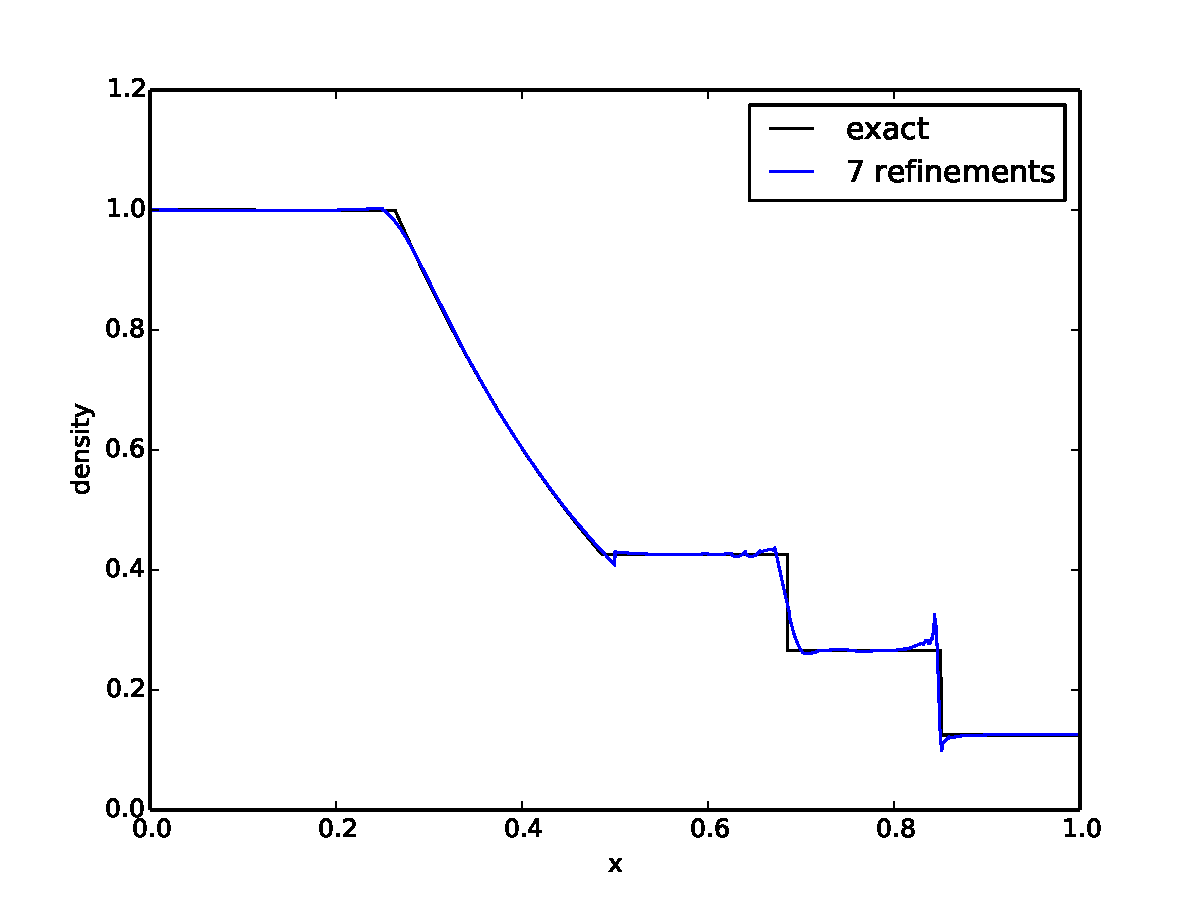
\includegraphics[width=\textwidth]{SpaceTimeCNS/Sod1e-5/den8.pdf}
\caption{Density after 7 refinements}
\label{fig:sod_den7}
\end{subfigure}
\begin{subfigure}[c]{0.3\textwidth}
\centering
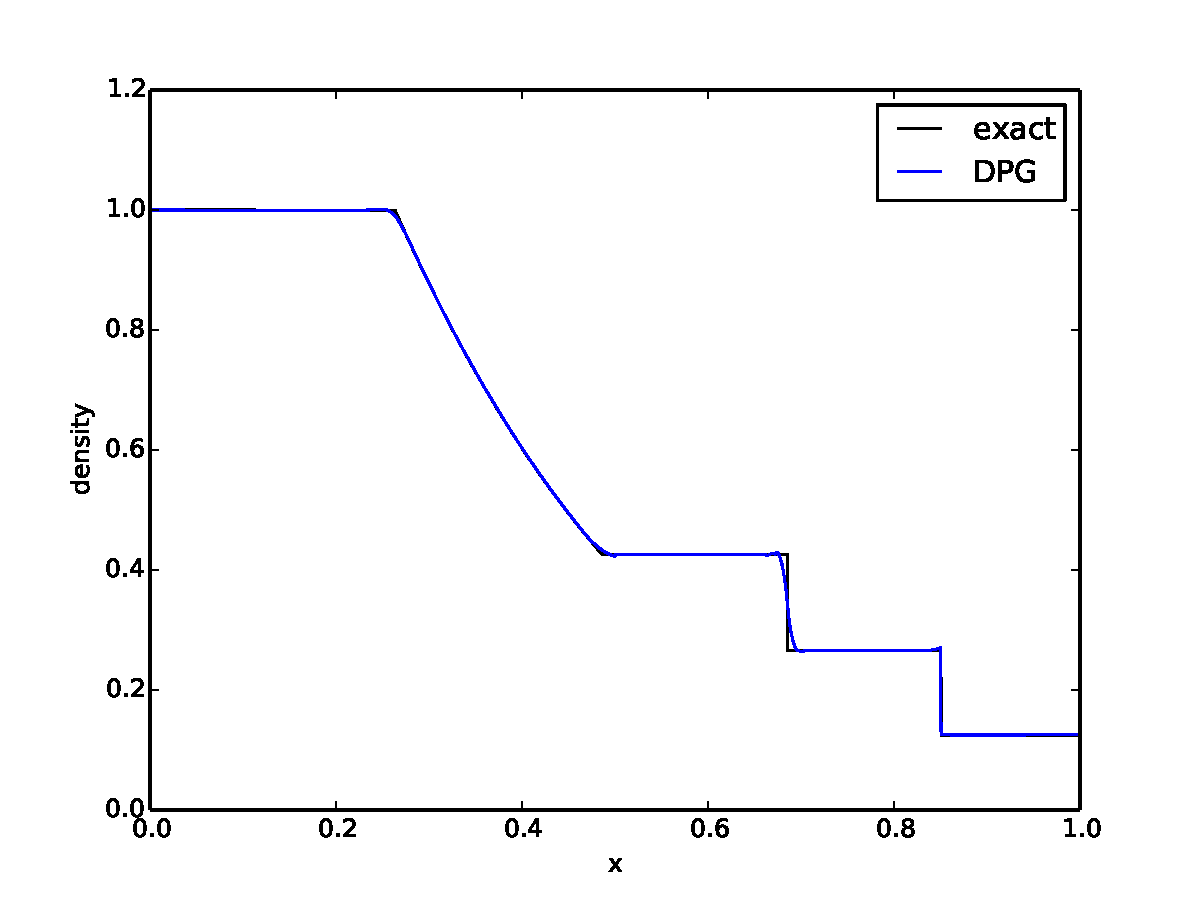
\includegraphics[width=\textwidth]{SpaceTimeCNS/Sod1e-5/den15.pdf}
\caption{Density after 14 refinements}
\label{fig:sod_den14}
\end{subfigure}
\begin{subfigure}[c]{0.3\textwidth}
\centering
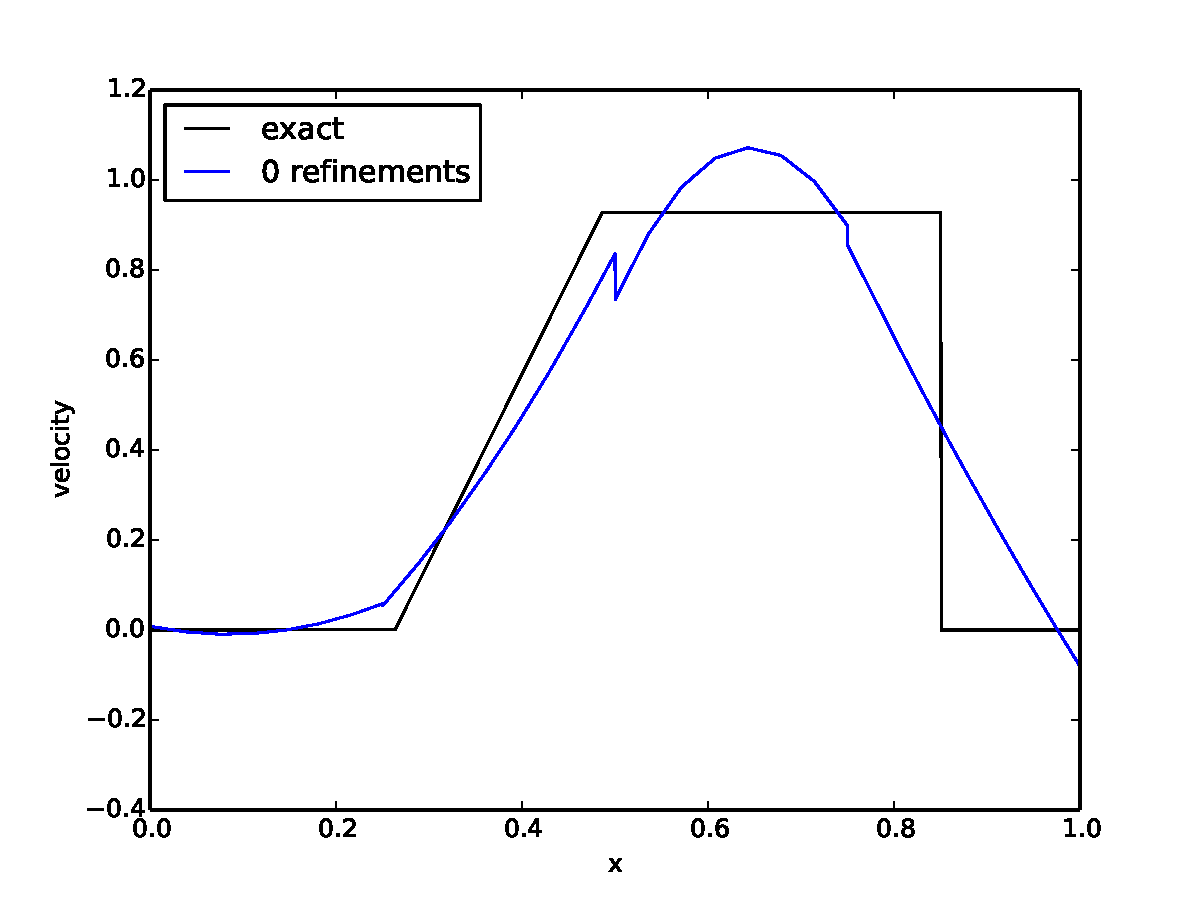
\includegraphics[width=\textwidth]{SpaceTimeCNS/Sod1e-5/vel1.pdf}
\caption{Velocity on initial mesh}
\label{fig:sod_vel0}
\end{subfigure}
\begin{subfigure}[c]{0.3\textwidth}
\centering
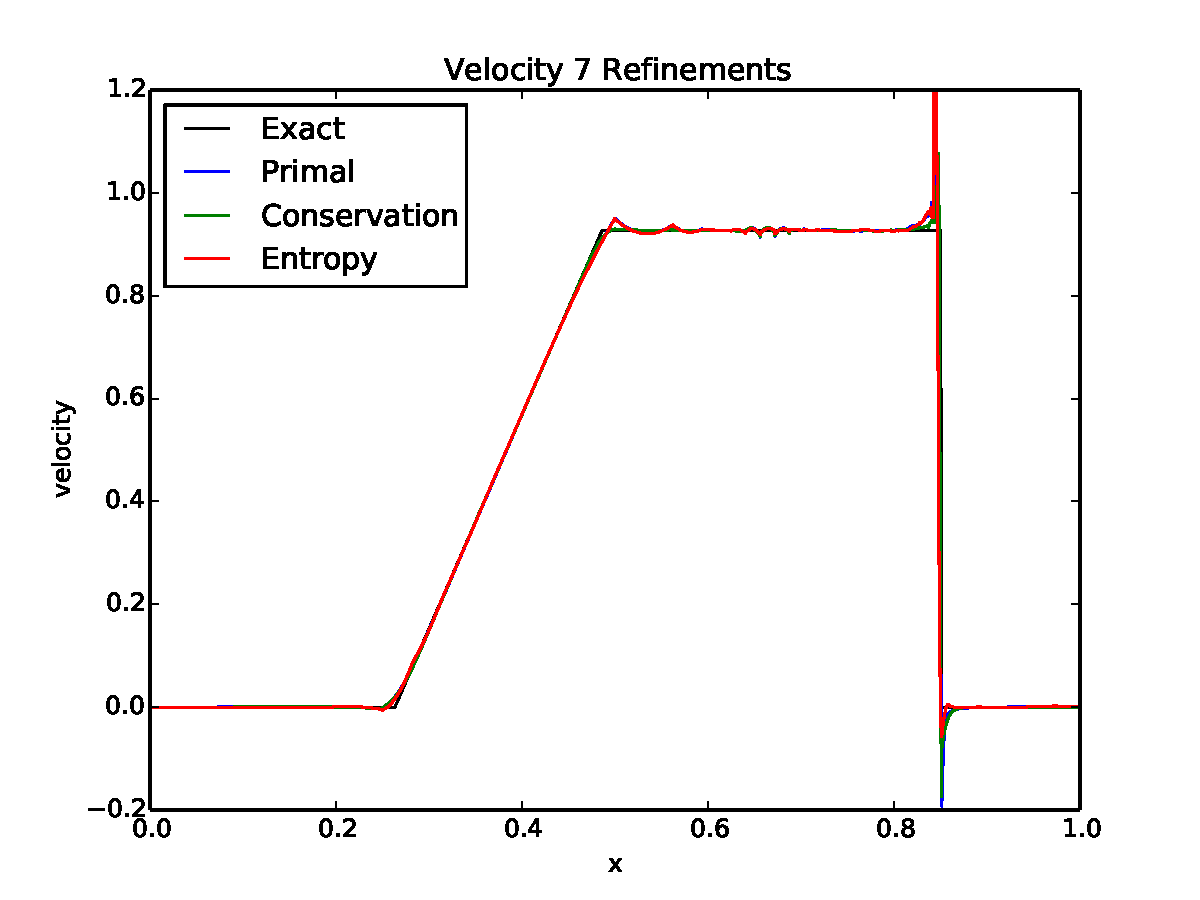
\includegraphics[width=\textwidth]{SpaceTimeCNS/Sod1e-5/vel8.pdf}
\caption{Velocity after 7 refinements}
\label{fig:sod_vel7}
\end{subfigure}
\begin{subfigure}[c]{0.3\textwidth}
\centering
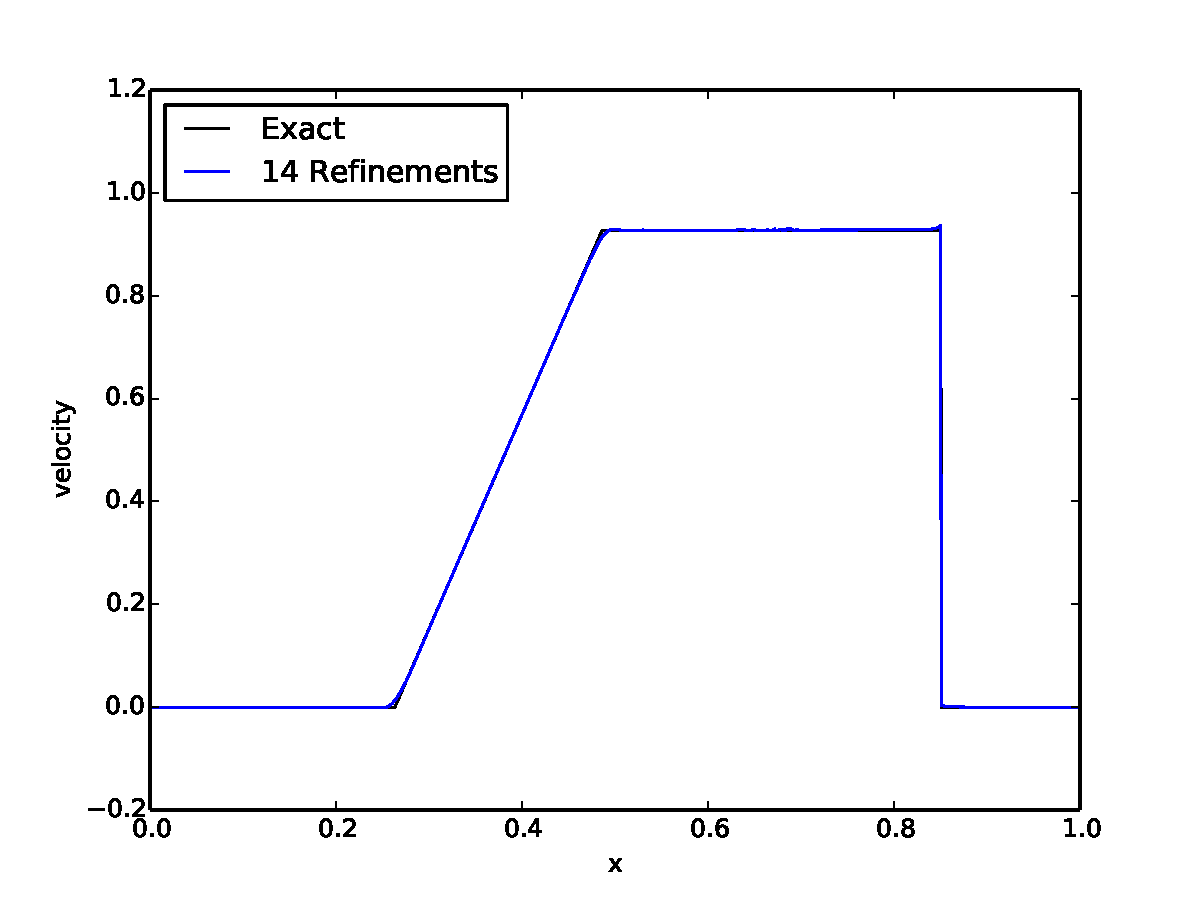
\includegraphics[width=\textwidth]{SpaceTimeCNS/Sod1e-5/vel15.pdf}
\caption{Velocity after 14 refinements}
\label{fig:sod_vel14}
\end{subfigure}
\begin{subfigure}[c]{0.3\textwidth}
\centering
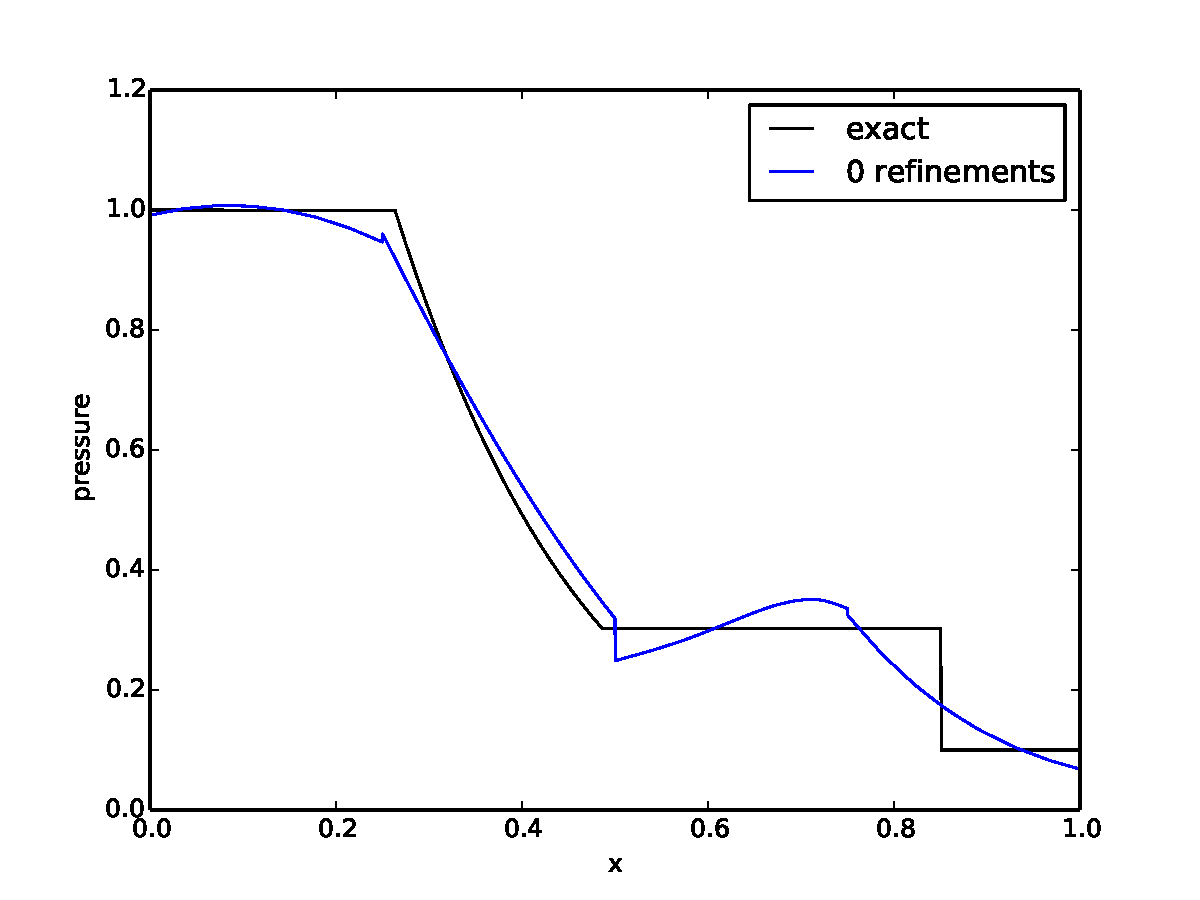
\includegraphics[width=\textwidth]{SpaceTimeCNS/Sod1e-5/pres1.pdf}
\caption{Pressure on initial mesh}
\label{fig:sod_pres0}
\end{subfigure}
\begin{subfigure}[c]{0.3\textwidth}
\centering
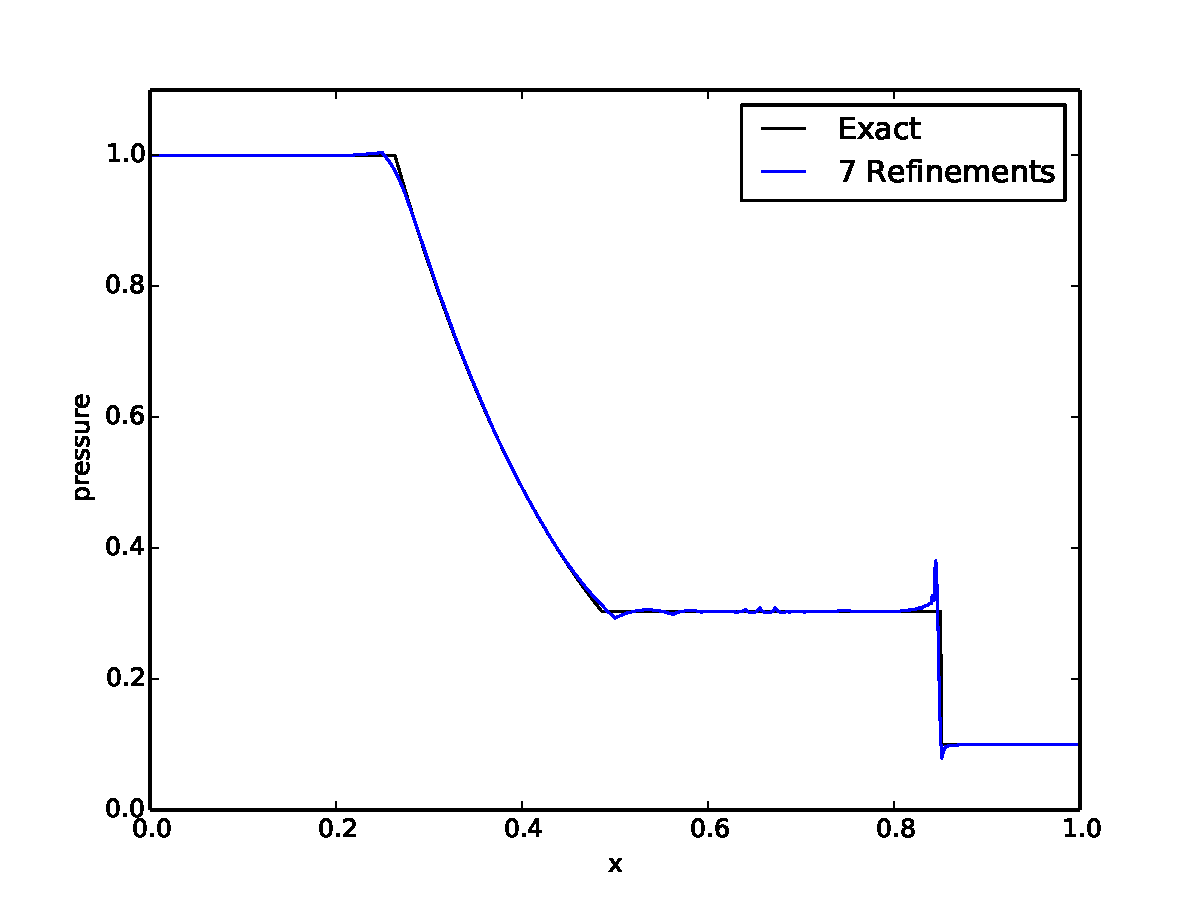
\includegraphics[width=\textwidth]{SpaceTimeCNS/Sod1e-5/pres8.pdf}
\caption{Pressure after 7 refinements}
\label{fig:sod_pres7}
\end{subfigure}
\begin{subfigure}[c]{0.3\textwidth}
\centering
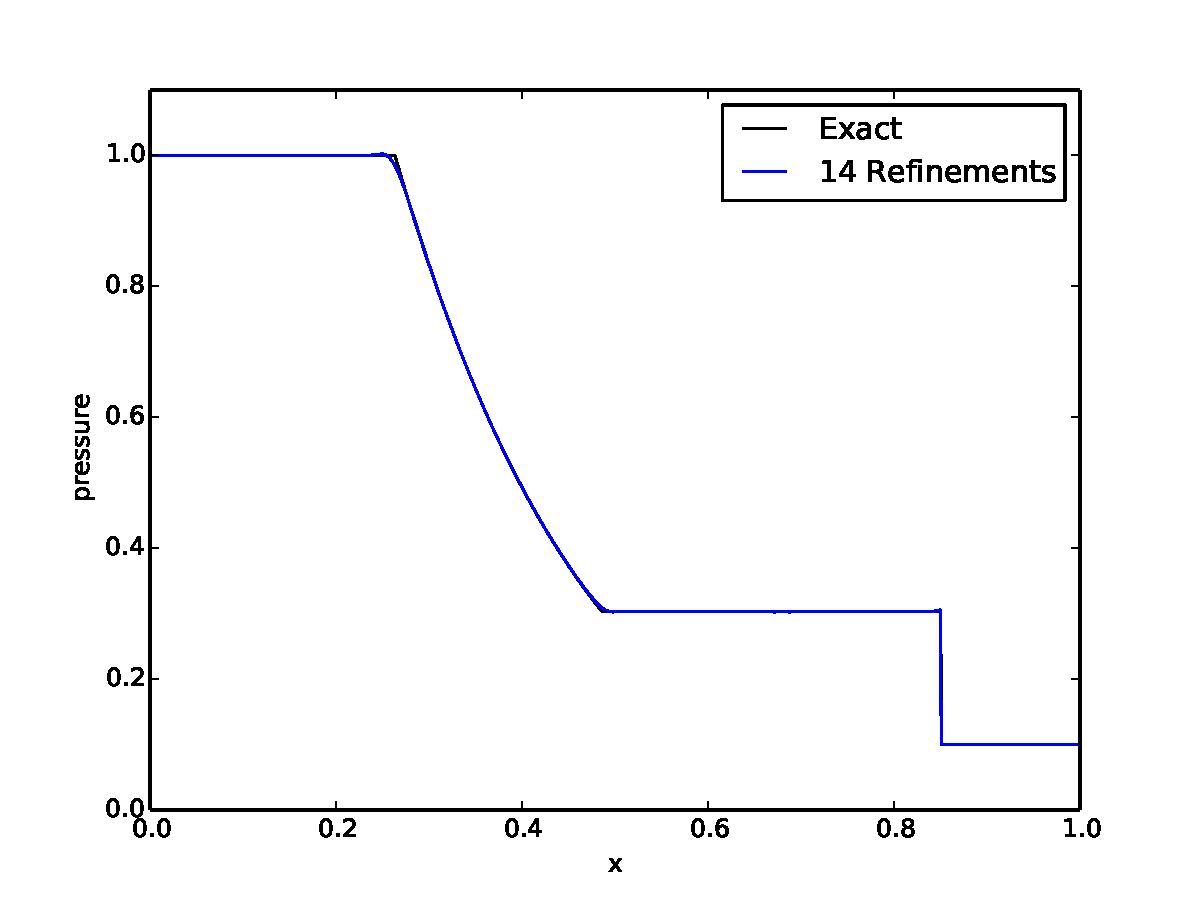
\includegraphics[width=\textwidth]{SpaceTimeCNS/Sod1e-5/pres15.pdf}
\caption{Pressure after 14 refinements}
\label{fig:sod_pres14}
\end{subfigure}
\begin{subfigure}[c]{0.45\textwidth}
\centering
\includegraphics[width=\textwidth]{SpaceTimeCNS/Sod1e-5/mesh1.png}
\caption{Density with initial mesh}
\label{fig:sod_mesh0}
\end{subfigure}
\begin{subfigure}[c]{0.45\textwidth}
\centering
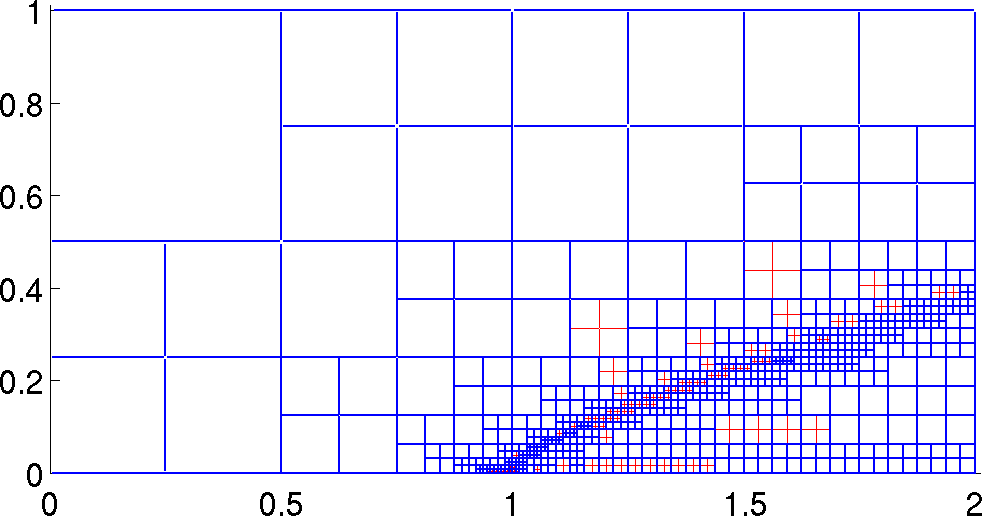
\includegraphics[width=\textwidth]{SpaceTimeCNS/Sod1e-5/mesh8.png}
\caption{Density with mesh after 7 refinements}
\label{fig:sod_mesh7}
\end{subfigure}
\begin{subfigure}[c]{0.9\textwidth}
\centering
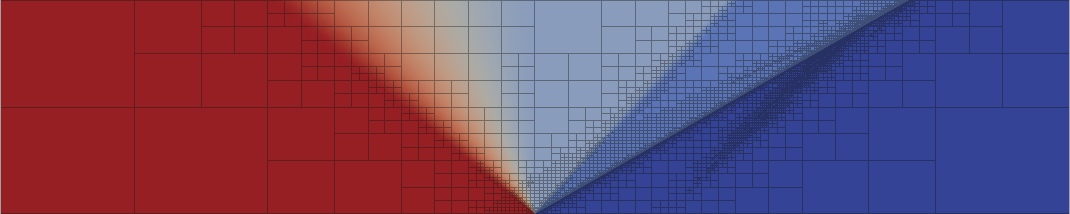
\includegraphics[width=\textwidth]{SpaceTimeCNS/Sod1e-5/mesh15.png}
\caption{Density with mesh after 14 refinements}
\label{fig:sod_mesh14}
\end{subfigure}
\caption{Sod problem with final time $t=0.2$}
\label{fig:sod}
\end{figure}

\subsubsection{Noh Implosion}
The Noh implosion problem\cite{Noh1987} is another standard test for Euler solvers.
The initial conditions are of an ideal gas with $\gamma=5/3$, zero pressure, uniform initial density of 1, 
and uniform velocity toward the center of the domain.
An infinitely strong shock propagates outward at a speed of 1/3.
For 1D flow, the post shock density jumps to 4.
We run this problem to a final time of $t=1.0$.
The longer time nature of this problem recommended the use of multiple time slabs rather than a single solve like the previous problem.
We run with four time slabs of thickness 0.25 each with 4 initial space-time elements.
We run the first slab to 8 adaptive refinements and set the initial conditions on the next slab to the refined solution on the previous slab.

Each of the slabs are put together into one long time solution in Figure~\ref{fig:noh}. 
Again we plot the solution on the initial mesh, a halfway resolved mesh, and a final mesh after 8 refinement steps.
We get some very odd behavior around the shock on the middle mesh, but this goes away by the final mesh.
We see the same behavior with overshoots and undershoots that we saw with the Sod problem. 

\begin{figure}[p]
\centering
\begin{subfigure}[c]{0.3\textwidth}
\centering
\includegraphics[width=\textwidth]{SpaceTimeCNS/Noh1e-3/den1.pdf}
\caption{Density on initial mesh}
\label{fig:noh_den0}
\end{subfigure}
\begin{subfigure}[c]{0.3\textwidth}
\centering
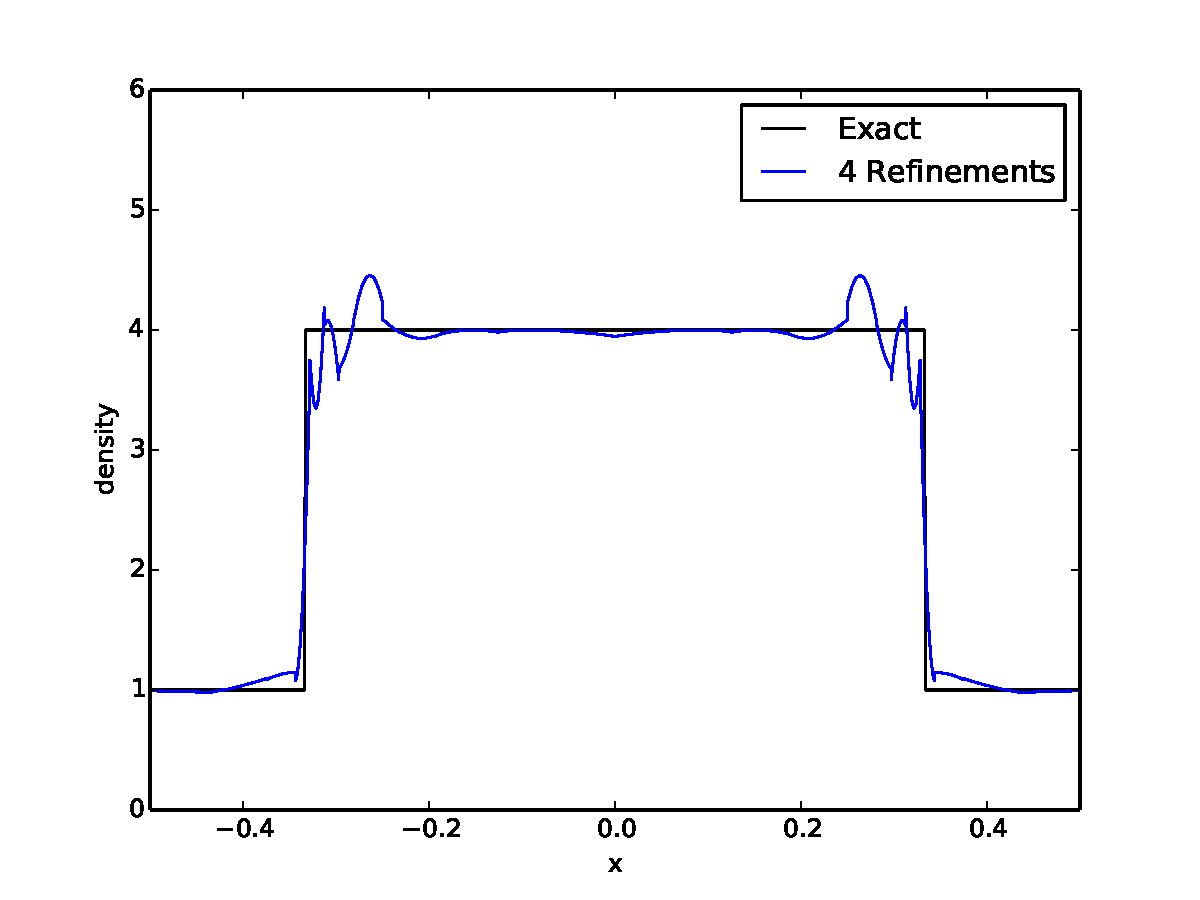
\includegraphics[width=\textwidth]{SpaceTimeCNS/Noh1e-3/den5.pdf}
\caption{Density after 4 refinements}
\label{fig:noh_den4}
\end{subfigure}
\begin{subfigure}[c]{0.3\textwidth}
\centering
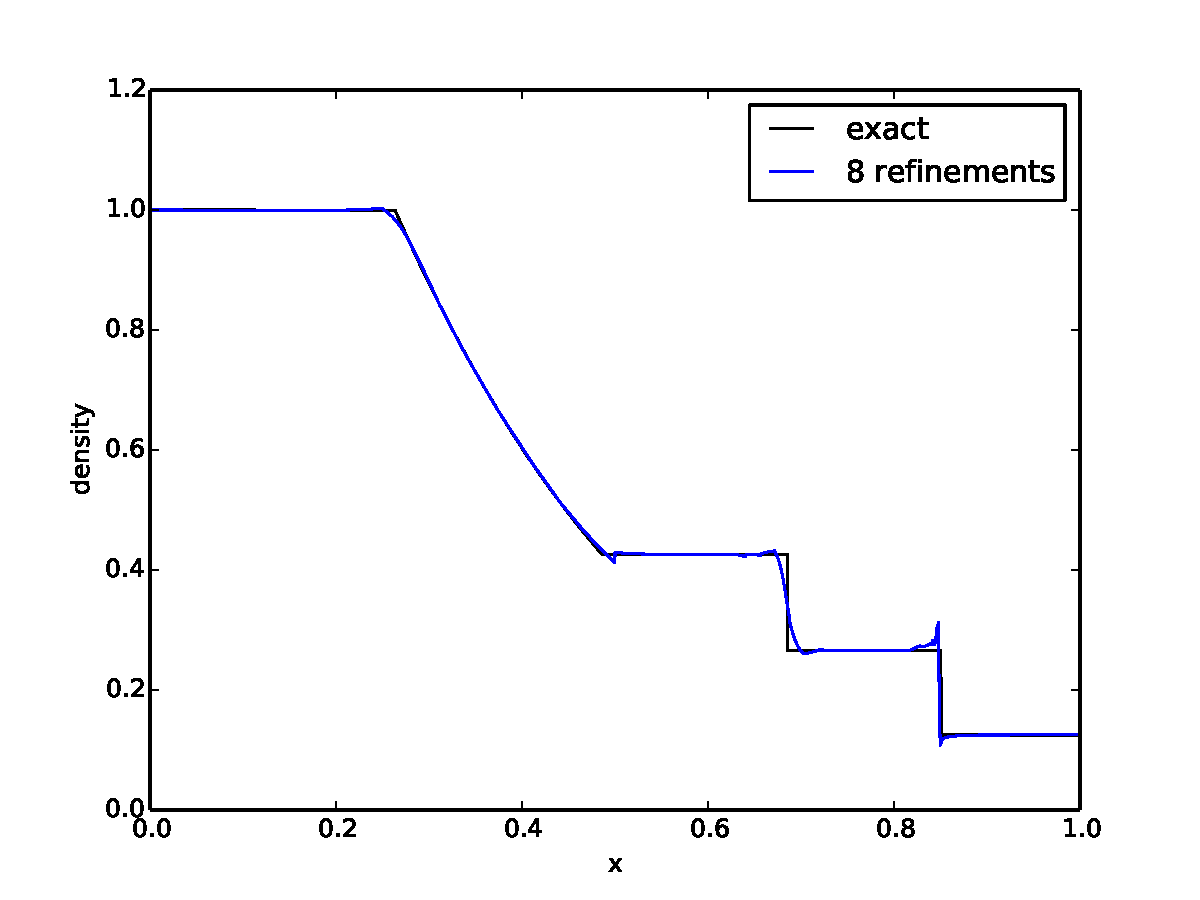
\includegraphics[width=\textwidth]{SpaceTimeCNS/Noh1e-3/den9.pdf}
\caption{Density after 8 refinements}
\label{fig:noh_den8}
\end{subfigure}
\begin{subfigure}[c]{0.45\textwidth}
\centering
\includegraphics[width=0.65\textwidth]{SpaceTimeCNS/Noh1e-3/mesh1.png}
\caption{Density with initial mesh}
\label{fig:noh_mesh0}
\end{subfigure}
\begin{subfigure}[c]{0.45\textwidth}
\centering
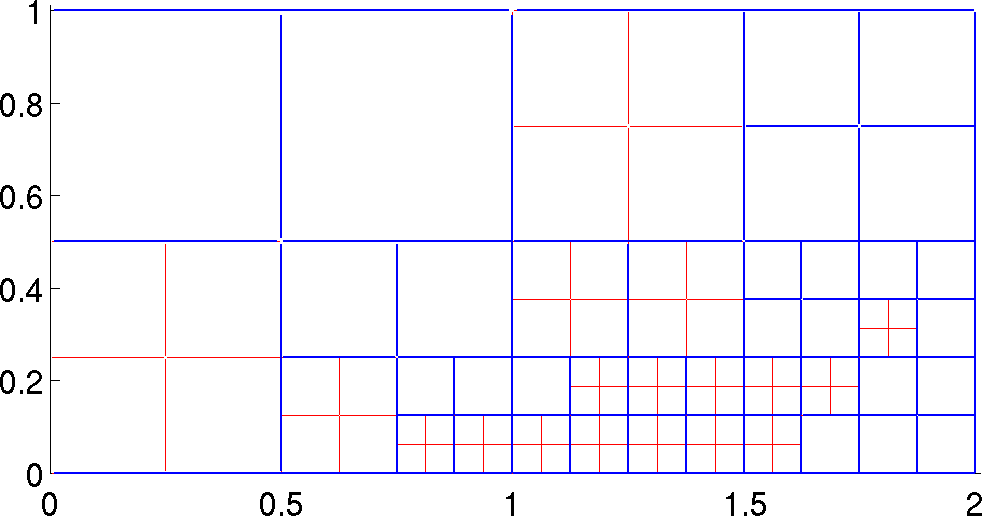
\includegraphics[width=0.65\textwidth]{SpaceTimeCNS/Noh1e-3/mesh5.png}
\caption{Density with mesh after 4 refinements}
\label{fig:noh_mesh4}
\end{subfigure}
\begin{subfigure}[c]{0.9\textwidth}
\centering
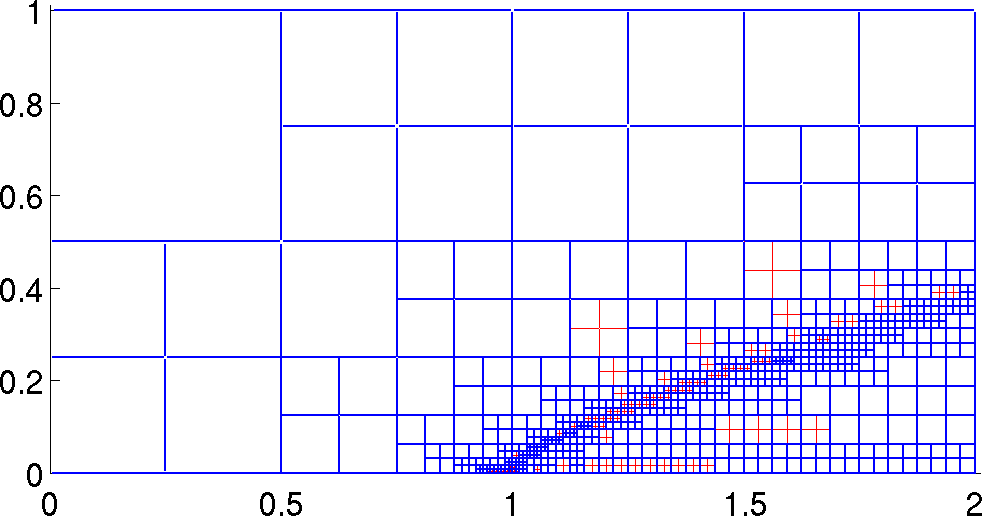
\includegraphics[width=0.65\textwidth]{SpaceTimeCNS/Noh1e-3/mesh9.png}
\caption{Density with mesh after 8 refinements}
\label{fig:noh_mesh8}
\end{subfigure}
\caption{Noh problem with final time $t=1.0$}
\label{fig:noh}
\end{figure}

\end{document}